%%% Version 2.1 Generated 2013/10/17 %%%
%%% You will need to have the following packages installed: datetime, fmtcount, etoolbox, fcprefix, which are normally inlcuded in WinEdt. %%%
%%% In http://www.ctan.org/ you can find the packages and how to install them, if necessary. %%%

%\documentclass{frontiersENG} % for Engineering articles
%\documentclass{frontiersSCNS} % for Science articles
\documentclass{frontiersMED} % for Medicine articles

\usepackage{url,lineno,listings}
\linenumbers

\lstset{ %
language=C++,                % choose the language of the code
basicstyle=\footnotesize,       % the size of the fonts that are used for the code
numbers=right,                   % where to put the line-numbers
numberstyle=\footnotesize,      % the size of the fonts that are used for the line-numbers
stepnumber=1,                   % the step between two line-numbers. If it is 1 each line will be numbered
numbersep=5pt,                  % how far the line-numbers are from the code
backgroundcolor=\color{white},  % choose the background color. You must add \usepackage{color}
showspaces=false,               % show spaces adding particular underscores
showstringspaces=false,         % underline spaces within strings
showtabs=false,                 % show tabs within strings adding particular underscores
frame=single,           % adds a frame around the code
tabsize=2,          % sets default tabsize to 2 spaces
captionpos=b,           % sets the caption-position to bottom
breaklines=true,        % sets automatic line breaking
breakatwhitespace=false,    % sets if automatic breaks should only happen at whitespace
escapeinside={\%*}{*)}          % if you want to add a comment within your code
}


% Leave a blank line between paragraphs in stead of using \\

\copyrightyear{}
\pubyear{}

\def\journal{Neuroinformatics}%%% write here for which journal %%%
\def\DOI{}
\def\articleType{Methods}
\def\keyFont{\fontsize{8}{11}\helveticabold }
\def\firstAuthorLast{Lowekamp {et~al.}} %use et al only if is more than 1 author
\def\Authors{Bradley Lowekamp\,$^{1,2,*}$, David T. Chen\,$^{1,2}$, Luis Ibanez\,$^3$ and Danial Blezek\,$^4$}
% Affiliations should be keyed to the author's name with superscript numbers and be listed as follows: Laboratory, Institute, Department, Organization, City, State abbreviation (USA, Canada, Australia), and Country (without detailed address information such as city zip codes or street names).
% If one of the authors has a change of address, list the new address below the correspondence details using a superscript symbol and use the same symbol to indicate the author in the author list.
\def\Address{$^{1}$Office of High Performance Computing and Communications, National Library of Medicine, National Institutes of Health, Bethesda, MD, USA \\
$^{2}$Medical Science and Computing, Rockville, MD, USA \\
$^{3}$Kitware Inc., Clifton Park, NY, USA \\
$^{4}$Mayo Graduate School of Medicine, Biomedical Engineering Department, Rochester, MN, USA}
% The Corresponding Author should be marked with an asterisk
% Provide the exact contact address (this time including street name and city zip code) and email of the corresponding author
\def\corrAuthor{Bradley Lowekamp}
\def\corrAddress{Office of High Performance Computing and Communications, National Library of Medicine, 8600 Rockville Pike, Bethesda, 20894, MD, USA}
\def\corrEmail{blowekamp@mail.nih.gov}

% \color{FrontiersColor} Is the color used in the Journal name, in the title, and the names of the sections.


\begin{document}
\onecolumn
\firstpage{1}

\title[The Design of SimpleITK]{The Design of SimpleITK}
\author[\firstAuthorLast ]{\Authors}
\address{}
\correspondance{}
\extraAuth{}% If there are more than 1 corresponding author, comment this line and uncomment the next one.
\topic{}% If your article is part of a Research Topic, please indicate here which.

\maketitle

\begin{abstract}

%%% Leave the Abstract empty if your article falls under any of the following categories: Editorial Book Review, Commentary, Field Grand Challenge, Opinion or specialty Grand Challenge.
\section{}
SimpleITK is a new interface to the Insight Segmentation and
Registration Toolkit (ITK) designed to facilitate rapid prototyping, education
and scientific activities, via high level programming
languages. ITK is a templated C++ library of image processing
algorithms and frameworks for biomedical and other applications, and
it was designed to be generic, flexible and extensible. Initially, ITK
provided a direct wrapping interface to languages such as Python and
Tcl through the WrapITK system. Unlike WrapITK, which exposed ITK's
complex templated interface, SimpleITK was designed to provide an easy
to use and simplified interface to ITK's algorithms. It includes
procedural methods, hides ITK's demand driven pipeline, and provides a
template-less layer.   Also SimpleITK provides practical conveniences
such as binary distribution packages and overloaded operators. Our
user-friendly design goals dictated a departure from the direct
interface wrapping approach of WrapITK, towards a new facade
class structure that only exposes the required functionality, hiding
ITK's extensive template use. Internally SimpleITK utilizes a manual
description of each filter with code-generation and advanced C++
meta-programming to provide the higher-level interface, bringing the
capabilities of ITK to a wider audience. SimpleITK is licensed as
open source software under the Apache License Version 2.0 and more information
about downloading it can be found at http://www.simpleitk.org.

\tiny
%All article types: you may provide up to 8 keywords; at least 5 are mandatory.
 \keyFont{ \section{Keywords:}  software design, Insight Toolkit, segmentation, interactive, software development, Image Processing   Software, image processing and analysis }
\end{abstract}

\section{Introduction}
The proper practice of the scientific method requires the systematic
verification of reproducibility of published reports
\cite{Popper1934}. Ideally, this verification should be performed by
independent observers for it to be trustable \cite{Popper1968}. In
the context of computational science, the reports of scientific
research must include the means and the complete details required to
enable independent groups to fully replicate the published results. 
In particular, they should include: data, reports,
list of experimental parameters, and software.

Open source software provides public implementations of state of the
art algorithms, that facilitate the accelerated advancement of a
field, through a more efficient research lifecycle and more
practical education. The National Library of Medicine's Insight
Segmentation and Registration Toolkit (ITK) is a leading open source
software for biomedical image analysis. Since 1999, it has been used
in fields as diverse as brain registration for neuroscience, microscopy
image analysis, radiation treatment planning, image segmentation for
brain tumors, and processing of electron microscopy, as well as
non-medical applications such as satellite imagery and industrial
inspection.

Our fundamental goal in developing SimpleITK was to grow the user community
of ITK.  Whereas direct use of the ITK programming interface requires
expertise in templated C++, SimpleITK was designed to be accessible
from a variety of higher level languages.  Furthermore SimpleITK has a
straightforward interface that requires no knowledge of the
intricacies of ITK's templated types. By lowering the bar to access
ITK's portfolio of image processing algorithms we hope to reach the domain
scientist and to further the goals of open source and open science.

\subsection{The Insight Segmentation and Registration Toolkit}

The Insight Segmentation and Registration Toolkit (ITK) was originally
conceived as open software tools for the analysis of the Visible
Human Project by the National Library of Medicine (NLM) with
partnership from six other institutes at the National Institutes of
Health (NIH). During the initial development the mission of ITK was
outlined as: “a software foundation for future research, an archival
repository of image processing algorithms, a catalog of validation
techniques, as well as a platform for advanced product development”
\cite{Yoo2002}. NLM has continued to support ITK through Algorithm Adaptors
and Data Distribution (A2D2) programs and on going maintenance, while
trying to foster the development of a sustainable open source
community. In 2010 NLM initiated a major revision and refactoring of
the toolkit funded by the American Recovery and Reinvestment
Act. Among the objectives outlined is to simplify ITK.

Through the contributions of the ITK community and continued funding
the scope of ITK has continued to grow. The version 4 refactoring
separated ITK into a modular structure which now contains over 100
modules. The segmentation algorithms available in ITK include region
growing, level sets, Markov random field classifiers, watersheds and
other statistical classifiers. The registration framework is designed
to be modular with the distinct parts for a transform, interpolator,
transform, optimizer, and image similarity metric along with support
for multi-resolution methods. ITK also contains data-structures for
spatial object, histograms, finite element meshes, quad-edge meshes,
neural networks, images and narrow band level-sets. There are a large
number of third party libraries that are supported and used for input
and output. Additionally there are a numerous image filters algorithms
available including mathematical morphology, smoothing, deconvolution,
distance maps, fast marching, image fusion, image statistics,
geometric filters, and image sources among many others. ITK contains a
wealth of algorithms, interfaces and data-structures to provide a
platform for research in algorithm development and a collection of
image processing algorithms.

The design of ITK focuses on providing a powerful and flexible
platform to allow for research, experimentation and development of
algorithms. To that end one of the notable implementation details in
ITK is the extensive use of C++ templates. The ITK image class is a
templated structure over both the pixel type as well as the image
dimension. This design choice pervades all areas of the toolkit. Image filters
must be templated over the image type. Also the data structures and objects
used with the image classes are templated. These structures
include image iterators, points, and indices. The results of this
interface design can be seen code listing \ref{lst:01}, taken from the
ITK Software Guide \cite{Ibanez2005}.

\lstinputlisting[firstline=36, lastline=74, label=lst:01, caption={A
    typical ITK example with templates, which reads an image, runs a
    Gaussian convolution then writes it back out to disk.}]{itkGaussianExample.cxx}

Notably missing from the design goals of ITK were usability and ease of
accessibility.


\subsection{WrapITK}

The native wrapping of ITK is performed with a project called WrapITK
\cite{Lehmann2006}, which was integrated with version 4 into the main source
repository. Its goal was to be a direct mapping of ITK's interface for
languages such as Python, Java and Tcl. As a direct mapping it
attempts to expose all of ITK's functionality including the pipeline,
template parameters of data objects and filters along with ITK's use
of pointers to objects. WrapITK provides interfaces to many basic ITK
objects such the basic array, index vector, point and matrix
classes. Additionally interfaces to the core data object types such as
images and transforms are provided along with iterators and other
utility classes. Most of these types have template parameters for both
dimension and value type. The available types in WrapITK make it
possible to use most of ITK's filters and many of ITK's modular
frameworks, such as registration, with the native ITK class to specify
parameters.

WrapITK's implementation was an evolution of the initial ITK wrapping
system which used CABLE \cite{Lehmann2006}. There are four components to
this system CMake \cite{Martin2003}, GCC\_XML (http://www.gccxml.org), pygccxml, and SWIG
\cite{Beazley2003}. The process is driven by CMake which runs GCC\_XML to
produce an easily parsable description of the ITK source code, then
uses manually written CMake ``wrap'' files along with Python's pygccxml
module to create a SWIG interface file and describe how the ITK
templates parameters should be defined. Next SWIG generates the C++
code which instantiates and wraps the ITK for the targeted language.

The result is a powerful exposure of ITK interface, along with many of
ITK's difficulties and problems. Each templated ITK class is
instantiated, compiled and wrapped as separate objects. So in the
target language the correct template parameters must be provided as
part of the class's name to be constructed. While this approach is
very much in the style of ITK, many of the targeted languages are
scripted and typeless, making this extra verbosity unnatural and
cumbersome.  This approach also has a very large impact on the size of
the WrapITK library and the number of symbols in the library. For
every ITK class, with every combination of template parameter, for
each method a wrapper method is needed, which introduces multiple
symbols in the library that must be loaded into the target language
namespace. With most of the pixel types instantiated, the WrapITK
library can be over a gigabyte, can contain nearly 3 million symbols,
and can take over a minute to load into Python. Also because of the size,
the large number of configuration options, and the compile-time and
configuration options, precompiled binaries are not available.

\subsection{Other Wrapping}
ManageITK was developed \cite{Mueller2007} to provide
wrappers for ITK for the .NET languages such as C\#, VB.NET and
IronPython. It was based on the WrapITK infrastructure, without the
use of GCC\_XML or SWIG, instead relying on a manual description of
properties of ITK classes, with the addition of some manually written
wrapper classes for key data types. Many of the advantages of this
interface come from the power of .NET including rapid GUI development,
support for multiple languages, and object browsing in an
IDE. However, this wrapping approach only works with Microsoft Visual
Studio on the Windows operating system, and properties and methods for
a new ITK object need to be manually added and updated.  Also there is
no testing generated for the wrapped interface.

MATLAB  (Mathworks, Natick, MA) is a popular commercial platform for research and
prototyping bio-medical image processing and other numeric computation
algorithms. There are several libraries available to access ITK
algorithms inside MATLAB, although they are not providing a direct
access to the ITK interface. These include MatITK\cite{Chu2006} and
SimITK\cite{Dickinson2011}.

\section{Design Goals}

SimpleITK is designed to reduce the burden of usage and expand the ITK
user community by simplifying the complexities that are frequently
encountered when trying to use ITK. Our goal is to expose the
algorithms in ITK in a readily available format. Currently a direct
ITK user must be a sophisticated developer with computer science
skills to be able to compile and combine ITK algorithms with their own
C++ code. While applications (Osirix, Paraview, SNAPITK, 3D Slicer)
are built on top of ITK, internally using ITK data structures and
algorithms and externally exposing certain filters for image
manipulation, users of these applications are not direct users of
ITK. We wish to expand the user base, by making the programming
interface accessible to non-computer scientists such as domain
scientists, biomedical engineers and mathematicians.

Interactive scripting and programming environments such as the
Python's SciPy environment \cite{Jones2001}, MATLAB
and The R Project for Statistical Computing are popular choices for
initial prototyping and experimentations. Scripting languages are
easily accessible to more people than C++.

The first complication a new user of ITK encounters is the lack of a
binary distribution or compiled software. They must download and
compile ITK from the source code, which requires development tools
such as a compilers and CMake which may be new to the user. This
requirement is a large initial hurdle, and problems are frequently
encountered as shown by the many help requests on the ITK community
mailing list.

A second common difficulty is dealing with the ITK's advanced C++
templates. ITK uses templates for both an image type's pixel type and
the dimension, and the algorithms are templated over the image
types. The naive usage of these features require the developer to
determine static types used at compile type.  The code required to
create a basic program is excessively long and verbose with basic
programs requiring numerous C++ type definitions.  If multiple pixel
types or image types need to be handled, then even more bulky and
complicated code require.

A third problem is complications arising from the ITK pipeline. When
filters in a pipeline get executed, the number of times they get
executed, and the implicit buffering occurring between filters can all
result in performance issues. Common problems include data or
meta-data being out of date, excessive memory usage due to filters
buffering output, and unnecessary re-execution of filters. In many
cases a naively assembled ITK data pipeline can perform worse than
sequentially executing filters.


\subsection {Survey and Architectural Review Board}
Kitware conducted a survey of the ITK and related computer vision and
medical imaging communities. A variety of mailing lists were query for
users to voluntarily fill out a survey including ITK, VTK, R imaging
group, LinkedIn, etc. Feedback was obtained on commonly used tools,
applications and requirements for image processing. There were 253
total participants of which 45 participants had never used ITK and 54
were uncomfortable using C++.

The survey produced several important conclusions. First, a ready to
use package greatly increases the likelihood of it being used. Second,
1 dimensional images are not important with only 4 participants saying
it would likely to be used. Third, for each pixel type the group was
asked to rate it's priority from ``Not important'' to ``Essential''. Every
pixel type had a minimum of 25\% of the participants saying it was at least
a ``High Priority''.

When asked questions about preferred programming languages,
programming styles, object oriented versus procedural, features of ITK
used or resource requirement, there was a lack of clear consensus. So
we concluded that it is important for SimpleITK to be flexible in its
usage.

To obtain more specific guidance on the design an Advisory Review
Board (ARB) was assembled consisting of 9 members from academia,
corporations and government agencies. During the design process pseudo
code of interfaces were reviewed. The ARB was another important voice
in the design process, giving opinions on best approaches and guidance
on prioritizing design philosophies.

\subsection{Goals}
For a successful project there are certain software engineering goals
that must be achieved for maximum impact. Firstly, the software must to appeal
to the greatest audience possible. This goal suggests that we must be
cross platform and support modern desktop operating systems such as
Microsoft Windows, Apple OS X, and GNU Linux. As observed in our
survey, a variety of languages should be supported and the framework
should easily be extendable to other target languages. Additionally,
to make it easiest for potential users to try the software there should
be binary downloads available.

Reliability and quality of the software is also of high importance. If
a potential user downloads the software, and the first thing they try
does not work, they may never invest the time to resolve the issue. To
achieve reliability, automatic and manual testing is a must. The
coverage of the code needs to be high to build confidence in the
quality and reliability of the software.

Given that we want to expand the ITK community beyond those who are
comfortable with the current complexities of ITK, certain features
should be hidden to enable clearer access to the core algorithms
available in ITK. A common complaint about ITK is the
difficulties with using the templates for image and filter algorithms. To address this an
important objective is to present a template-less abstraction  or
“typeless layer” to the native ITK interface which implicitly handles
the ITK templated types. We set the larger goal of not exposing any
templates in the SimpleITK interface.

Another challenge in our design is to provide a procedural interface
to the algorithms, while still providing a object oriented for those
that prefer it. Therefore the interface design needs to be flexible so
that it can support multiple usage styles.

There are many aspects of ITK that we would like to retain. The
algorithms still needed to be at the high performance standard that
ITK currently has as a compiled C++ library. And we still would like
support for the flexible multi-threaded infrastructure when the
filtering algorithms are executed. The survey participants placed a
high priority on the large number of pixel types available in
ITK. Therefore we must support this wide variety of pixel types
including color images and vector component images.

The initial mission of ITK included providing a platform for algorithm
development, SimpleITK goals focus on providing usable algorithms. So
the building block that ITK provides for algorithm development such an
image iterator, adaptor, neighborhood algorithms and other utilities
and interfaces are not designed to be included in the SimpleITK
interface. This will not exclude SimpleITK from being a platform where
new algorithms can be developed. For example new methods can be
developed that are a composite of other algorithms.

Lastly, while ITK is an biomedical segmentation and registration
library, it explicitly does not contain any visualization. That is a
user can not view an image with ITK alone. Viewing an image requires
an external program or library. However for SimpleITK to be part of an
interactive environment convenient visualization of intermediate
images is required.

\section{Implementation}

We implemented SimpleITK as an interface on top of ITK, built as a C++
library. This interface is then wrapped for a variety of targeted
languages. The SimpleITK interface is functionally complete and fully
encapsulates ITK.  In other words SimpleITK can be used independently
without any direct calls to ITK. This interface was designed from the
ground up to be easy to use and intuitive, as well as to take
advantages of advanced language features and convenience.

The goals for this project were high, and some of them seemed in
conflict. The challenges of presenting a procedural interface for the
highly object oriented and templated ITK library while still
preserving robust support for multiple image dimensions and pixel
types was the essence of the problem in designing SimpleITK. Based on
our motivations and goals a number of choices were made.

\subsection{Decisions}
\subsubsection{No exposed pipeline}
One of the first decisions was that we were not going to expose ITK's
demand driven pipeline. We decided to hide the pipeline because errors
in using the pipeline are quite common to new users. Without the
pipeline, results of operations are immediate so there is no chance
that an image is out of date or missing information. Users can simply
call the methods needed to set a filter's parameters then execute the
filter.  The overhead required to connect, manage and update filters
is removed from the interface. Also, with filters executing
immediately, the object oriented and the procedural interfaces can be
closely related.

\subsubsection{Use SWIG for Wrapping}
One of the fundamental goals of SimpleITK was to provide language
bindings for different languages such as Python, Java, C\#. Due to the
large number of language targets, a single unified tool for all
languages was required for maintainability. The Simplified Wrapper and
Interface Generator (SWIG), is open source and a powerful
development tool for wrapping C++ with numerous high-level programming
languages. SWIG has support for over 20 target languages. It is
capable of parsing basic C++ interfaces and generating glue code to
connect the target languages to the interface. The result is generally
a direct mapping of a methods from the target language to an
associated method in the C++ interface.

WrapITK uses SWIG to interface ITK with other languages.  But the
complexity of the templated programming used in ITK, means that SWIG
cannot directly wrap ITK.  Instead WrapITK requires additional tools
to explicitly specify the interface of ITK in a format that SWIG can
understand to wrap certain instantiations of the templated ITK
interface. SimpleITK's simplified interface is designed to be directly
wrappable by SWIG.

\subsubsection{Parameter Types}
ITK uses a variety of array-like types such as arrays, vectors,
indexes, sizes, points and offsets. These types have template
parameters such as dimension and value type which makes them dependent
on the type of the image, resulting in dozens of array-like types in
the native ITK interface. SWIG has built in support for many C++
Standard Template Library (STL) objects such as std::vector and
std::list and provides specialized interfaces for target
languages. For example SWIG can provide an interface to a std::vector
in Python similar to its own list or tuple type along with implicit
conversions. This feature greatly improves the interaction in the
target language, giving the interface a native feel. Because of the
goal to create a template-less layer free from compile-time
parameters, SimpleITK uses std::vectors for array-like parameters for
its interface. However, for the targeted scripting language it may
appear as native arrays.

\subsubsection{Hide Smart Pointers}
Pointers and explicit memory management are elements of C++ that
preclude it from being considered a high-level language compared to
scripting languages like Python. The smart pointer design pattern is a
combination of implicit reference counting for objects along with an
interface of a standard pointer so that objects can be automatically
deleted when no longer referenced. Thus reducing the burden of explicit
memory management. While smart pointers are used in ITK, they are not
simple enough for SimpleITK as they may introduce a new concept in
target languages. Many languages provide a direct object type, not a
separate pointer type that refers to the object. The burden of a
direct approach in C++ is that implicit deep copies of objects occur
during assignments and passing arguments by value. We decided that
SimpleITK would provide direct image, filter and transformation
objects but not provide the undue burden of implicit copying.

\subsubsection{Template-less Layer}
The template-less or “typeless” layer concept's goal is to hide ITK's
template parameters from the user. A common suggestion was to simply
consider all images as 32-bit or 64-bit real numbers. However, this
approach can cause unacceptable memory use and performance
penalties. Consider starting with an image that is an 8-bit and 4
gigabytes.  Converting to a 64-bit type would use eight times the
memory now requiring 32 gigabytes of memory for its
representation. This monolithic choice changes the nature of working
with an image from one that can be done on a laptop to one that
requires a large server. Additionally, the users surveyed demanded the
flexibility to use a variety of pixel types.

Therefore the template-less layer concept requires that SimpleITK
images all have the same external type and interface, unlike ITK. The
details of dealing with the different ITK template parameters is
hidden so that the user can generically manipulate any image. An
image's pixel type and dimension are handled by SimpleITK internally
and not directly exposed to the user, unlike ITK which requires the
user to explicitly determine them at compile-time. At runtime a
PixelIDValue, in the form of an integer and enumerated type is used to
represent a pixel type, which along with the image dimension are
intrinsic run-time attributes of the SimpleITK image.

\subsubsection{Facade Interfaces}
The facade design pattern is a software design pattern to present the
user with an simplified interface to a larger body of code
\cite{Gamma1995}. This approach is how SimpleITK encapsulates ITK filters
and data objects, where  the body of code encapsulated is the set of
template parameters for a class. Our facades internally use ITK
objects and call ITK methods, so there is very little additional
code. The facade code provides a template-less layer to instantiate
and dispatch to the correct templated ITK code. Additional code is
used to make the objects of the facade behave natively instead of
requiring smart pointers and converting between the templated ITK
array-like types and STL objects.

\subsection{The Design of the SimpleITK Image}
The image class is at the heart of SimpleITK. It is the most commonly
used class and has been specially designed to provide a natural and
intuitive user interface across multiple target languages. We followed
our principles for intuitive interface driven design by writing
numerous example code blocks and discussing tradeoffs with the ARB.

From an interface perspective, the handling of the life of an object,
i.e. how the object is constructed, copy and destroyed, is a key
aspect of developing an intuitive interface. Because we chose not to
expose smart pointers, we are use a completely different approach from
ITK's New method. Our approach is simple and translates to other
languages seamlessly. We simply directly expose the image class's
constructors and destructor without the restrictions applied in
ITK. The reasons ITK uses the New factory method include: adding
flexibility to override a class' implementation and enforcing smart
pointers use by preventing stack based allocation. Our approach to the
SimpleITK interface does not allow our classes to be directly
overridden but still allows ITK class overrides to occur
internally. As we encourage the direct use of our image class, the
smart pointer motivation is mute as well. An image is able to be
default constructed, as an image of size zero. An image of any
dimension or pixel type is considered to be empty if its size is
zero. The common constructor methods take parameters for the size of
the image along with the pixel type and support the option for the
number of components per pixel. The dimension of the image is
determined by the number of components used for size. How images are
copied is closely related to their constructors, but the relationship
between the SimpleITK interface and ITK objects needs to be described
first.

The SimpleITK image interface presented, utilizes the facade design
pattern in conjunction with the private implementation, pimpl pattern
\cite{Sutter1999}. It is a facade in that it provides a unified interface
for multiple ITK class and template parameters. The single SimpleITK
image class provides an interface to ITK's Image, VectorImage, and
LabelMap classes and supports  multiple dimensions and pixel
types. However, the SimpleITK Image class is not polymorphic, i.e. it
is not a virtual base class and does not contain virtual
methods. Instead it relies on an internal pointer to a private class
in the pimpl pattern to provide a unified polymorphic interface to
ITK's image class. The pimpl image has an abstract base class for the
unified interface with templated derived classes to implement the
specifics. This pimpl image fully encapsulate ITK's templates and
instantiates all the ITK image classes. A call from the SimpleITK
interface to an ITK image is quite efficient and direct despite the
complexity of the patterns used. A call to the SimpleITK image's
method, calls the same method in the Pimpl Image through the
polymorphic interface, which then calls the ITK method. This dispatch
method is direct and free from any conditionals. The SimpleITK image
only contains a pointer to the pimpl image which only contains a smart
pointer to ITK image. This implementation provides an efficient
interface with low overhead.

Our interface also allows for direct copying and assignment of the
image class in an optimized manner. From a user perspective, the
availability of optimized copy methods is generally all that needs to
be known. However, we have optimized these methods by using a form of
lazy evaluation through a copy-on-write (COW)  policy. This policy is
a key component that allows for an efficient implementation while
removing pointers from the interface. Ironically, COW is implemented
by using ITK's smart pointers. When a copy of a SimpleITK image
occurs, a new ITK smart pointer to the image is create and
stored. This new smart pointer increases the reference count contained
of the ITK image. When there is a write request to the SimpleITK
image, the reference count is checked; if it is not 1, then a deep
copy is performed of the bulk image data. This approach enables the
SimpleITK image to be passed by value without the overhead of
implicitly copying the bulk image data.

Our user survey and ARB discussions were inconclusive in determining a
limited set of important pixel types to implement. As adding more
image or pixel types does not increase the number of methods in the
SimpleITK interface, we do not limit the types enabled. Currently we
have up to 26 different pixel types available including scalars,
multi-component vectors, complex as well as label maps implemented
with the run length encoded LabelMap classes. Fully implementing these
type does not have an adverse effect on usability or run-time. It does
however increase the demands on the system requirements for compiling
the library. As the goals for SimpleITK focus more on usability of the
interface then ease of building, it was determined to be a reasonable
tradeoff. Additionally, we settled for only supporting 2 and 3
dimensional images. Interest by the users in higher dimensional images
was limited.

The Image interface was also customized for C++, Python, R, Java and C\# to
provide additional syntactic enhancements to make language integration
as easy as possible. These enhancements include features such as
operator overloading, advance subscripting, and utilizing weak typing
of return values in many scripting languages.

The resulting image class provides a simple and easy to use interface
that fully encapsulates the complexities of ITK. Among the things that
are hidden include templates for both the image dimension and pixel
type as well as multiple image classes. Details such as
smart-pointers, memory management and copy semantics are also removed
and replace with a straightforward C++ interface. This standard
interface can be directly wrapped by SWIG, thus providing a
conventional interface for different target languages.

\subsection{The Design of the SimpleITK Filters}
Among the objectives which drove the filter interface design of
SimpleITK included removing the dependency on the image type at
compile-time, the removal of ITK's data driven pipeline as well as
providing a flexible interface which has an object oriented and
procedural interface. With the template-less image class designed and
the decision to use STL's std::vector as parameters whose length is
dependent on the image dimension, the interface was rather straight
forward. Determining which types to use for filter method parameters
was a difficulty when it was the same type as the image's pixel
type. Generically using the double type resolved this issue. The
double is a superset of all scalar pixel types except 64-bit integers,
and for vector pixel types the scalar value is replicated for all
components. Listing \ref{lst:02} can be used as a reference.

\lstinputlisting[label=lst:02, caption={A prototypical example of a
    SimpleITK filter interface.}]{filter.h}

In ITK, the pipeline needs to be explicitly updated before results can
be examined. This update initiates the examination of the dependencies
in the pipeline to determine the necessary filters to execute. After
the Update method of a filter is called the results in the output are
valid and can now be examined. Without the pipeline, a filter is
executed immediately, so the method name Execute was chosen to
illustrate the difference. Filters which have secondary results, such
as a number of iterations or a measurement of error are problematic
for the procedural interface as functions naturally only return a
single value. The solution was to add “measurements” only to the
filter classes. An alternative approach, to make these available
through the procedural interface was  have them as arguments to the
procedural methods. However doing so would result in too many
arguments, and passing by reference or pointer is not portable across
differing languages.

Defining the behavior of a filter is more complicated than specifying
the desired interface for the template-less filter. For each filter
decisions must be made about the input types supported as well as the
image type produced. The goal is to have filters support as many image
types as possible. Even when the ITK filter does not directly support
vector images, the SimpleITK infrastructure can execute the ITK filter
on each component independently. For determining the output image type
there are a couple general policies that occur. The first and most
common is defining the output image type the same as the input. This
is sensible for many filters including mathematical morphology, image
grid manipulations, and label image manipulations. For other filters
having a fixed output type is sensible. For example filters which
output a mask such as thresholding, always output a unsigned 8-bit
integer, while distance field filters produce 32-bit floating point
numbers. Consideration must include limiting the number of
instantiated filters of one type to a reasonable number, to prevent
excessive compilation and library size from excessive permutation, so
in general there is no selection of the output type.

Those filters which take two image as input required special
consideration for how to handle the multiple types. In ITK, filters
that are binary “functors” such as the addition and subtraction
operators, have 3 template parameters corresponding the two inputs and
the single output. This approach makes ITK very flexible by allowing
conversion to occur simultaneously with the operation. Languages have
different type promotions schemes, and certain overflow and
conversions are explicitly undefined in C++. Therefore we decided that
most of the binary filters require the inputs to both be of the same
type as well as the resulting output. So we do not do any implicit
conversion or promotion, thereby requiring the user to explicitly cast
the inputs to be the same type. SimpleITK does have the ability for
filters to accept multiple images of differing types and to use the
correct ITK filter templates based on these input types. These filters
are called “dual” image filters in SimpleITK. They have been used
sparingly due to size constraints when the computation validity of
multiple types is not in question.  The types of filters where this
feature is used include filters with masking and overlays. The group
of filters which allow the user to select the output type such as
casting, camping, and resample also use the “dual” dispatch
infrastructure.

By choosing to remove ITK's pipeline architecture from SimpleITK there
are numerous simplifications that we have taken advantage in our
design. Among the ITK features SimpleITK omits are the advanced
details of memory management occurring in the pipeline such as
releasing data, and running filters “in place”. They are not relevant,
since SimpleITK has an immediate execution model that lacks pipeline
buffering. ITK's interface for the ProcessObject, which is the basis
for all filters, consists of over 40 public methods for manipulating
the pipeline and managing the inputs and outputs. All these methods
are irrelevant for SimpleITK's Execute method approach. Omitting them
simplifies the interface for each filter class.  Among the features
still relevant is the monitoring of progress and events; these
features are scheduled for the next release of SimpleITK, version 0.8.

\subsection{Implementation Details}
The design of the interface was not done in isolation from the
implementation. Extreme software development methodologies were use to
continuously test and regularly integrate features into a stable
version.  The goals and the design of the interface presented immense
software engineering problems that had not been addressed before with
ITK. Initially there were doubts that maintainable code and
infrastructure could be developed to create a template-less layer for
a significant part of ITK's filters without unmaintainable, manually
created code. Our resulting implementation uses advanced C++ template
meta-programming to perform compile-time execution of code generation,
as well as traditional code generation based on the description of
filters. The details in this section are completely hidden from a user
of SimpleITK, and are relevant to those examining the internals of
SimpleITK or those who wish to learn the novel techniques used for
similar projects.

\subsubsection{Overview}
SimpleITK is implemented with more than just static code. It is a
complex sequence of code generation and compilation to produce the C++
interface, followed by wrapping with SWIG for the target
languages (See figure \ref{fig:01}). The manually written common code of SimpleITK consists of
the meta-programing infrastructure for the template-less layer and the
core data structures such as the image and the transform
classes. Also, a few of the filters and the reading, writing and image
display interfaces are written by hand. As of SimpleITK 0.7rc1, the
SimpleITK C++ interface for 245 image filters is automatically
generated from manually written descriptions.

\subsubsection{Code Generation}
After experimenting and iteratively improving manually written filter
interfaces, it was immediately apparent that a solely manually written
interface would take excessive time to develop, lead to an
inconsistent interface, and be unmaintainable. Due to the requirement
of maintaining a consistent interface among a large number of filters,
automatic source code generation became the natural choice. Code
generation allows the developers to focus on writing the generator and
the description at a higher level than the immediate interface.

Each generated filter in SimpleITK is described by a JavaScript Object
Notation (JSON) file. The JSON file structure is a lightweight data
format popularized by JavaScript programming for the web, which is
easy for both humans and computer software to read and write. The JSON
description contains the essence of an ITK filter. A filter
description contains expected named fields, such as \textit{name},
\textit{template\_type}, \textit{number\_of\_inputs},
\textit{pixel\_types}, and \textit{output\_pixel\_type}, with
values, as well as more generic fields which can contain C++ code to
be inserted into the template. The \textit{output\_pixel\_type} is
frequently more that just a static value by containing meta-programing
to transform the input type to the output. Additionally, there is the
\textit{member} sections which contains the description for each filter
parameter so that it can be stored in the SimpleITK facade and
translated into the typed ITK filter. There is also an optional
section to describe \textit{measurements}, and how to update the member
variable from the results of the ITK filter.

For normal image filters previously mentioned portion of the JSON
description can generally be written in just a few moments from a
similar example. The time consuming part in writing a JSON description
is the \textit{tests} section. This section contains input image file names,
the values of parameters, and either a hash of the expected output or
a baseline image to compare a test against. By including this section
we are able to generate tests for each language to verify usability
and functionality of the filter with different image types. Automatic
testing is critical to developing a robust interface that is proven
and reliable.

The generator of the source code is a text based program, which
processes a set of text inputs and produces source code. Lua is a
powerful, portable, fast, and lightweight scripting languages
\cite{Ierusalimschy2006}. We chose it as the language for the source code
generator script because its small size makes it easily included as
part of the SimpleITK source and compiled during the build
process. The generator script is derived from the Lua ``Text Template
Expand'' example (http://lua-users.org/wiki/TextTemplate) combined
with an publically available JSON  parser. This system uses template
files which contain and inlined Lua expressions all of which are
evaluated into strings. The scope of the Lua expressions include
variables from the current scope in the JSON description file. There
are template files for filters of types such as \textit{ImageSources},
\textit{BinaryFunctorFilters}, and \textit{DualImageFilters}.

\subsubsection{Template Meta-program and Typelists}
The crux of the problem for the template-less layer is the ability to
map the runtime pixel type information, PixelIDValue, available from
SimpleITK's image to the compile-time template parameters in ITK and
visa versa. Template meta-programming in C++ is the use of templates
to perform compile-time execution to generate code. SimpleITK uses a
concept called ``Typelists'' list to operate on list of types, PixelIDs,
which represent the types of pixels. Specifically these lists have
compile-time operations to append, merge, intersect, search, traverse
and perform permutations of selections from two lists
\cite{Alexandrescu2001}. The runtime ID of a pixel type, PixelIDValue, is
the index in the global InstantiatedPixelIDTypeList type, which is a
Typelist of all the available pixel types. There are a variety of
groups of PixelIDs declared as Typelists such as integer, real and
vector. The JSON description of a filter describes the valid input
pixel types by performing meta-programming operations on these
Typelists.

The compile-time mapping of the run-time PixelIDValue to an
instantiated function with the image as a template parameter is more
problematic. The compile-time mapping of the PixelID to the scalar
PixelIDValue can and must be done on all instantiated types. On the
other hand the templated functions can only be instantiated with the
parameters that are specified via Typelists. Otherwise the code may
not be valid.

The mapping of the run-time PixelIDValue to an instantiated member
function is done with an abstraction called a
MemberFunctionFactory. This factory has a method which maps a
PixelIDValue and image dimension to a member function pointer of an
instantiated member function over the associated ITK image
type(s). These functions are registered into the factory by passing a
PixelID Typelist and the dimension. Additionally the factory has a
templated object which knows how to get the address of  the member
function, enabling the compile-time traversal of the Typelist to
instantiate the member function.  With the member functions stored in
the factory, they are indexable by the PixelIDValue at run-time. This
MemberFunctionFactory is the heart of the dispatch system used to
implement SimpleITK's templateless layer and is an important software
engineering innovation for dispatching run-time mappings to ITK types.

\subsubsection{Automated Documentation}
Without documentation to accompany filters and algorithms, the
interface of SimpleITK would be unusable. Duplicating the effort to
describe each algorithm and parameters with what has already been done
in ITK would be a foolish task. Doxygen is the de facto standard tool
for generating reference manuals of a programming interface from
annotated source code (http://www.doxygen.org). It is used as the source code annotation
throughout ITK and SimpleITK. For all the manually written SimpleITK
infrastructure and facade interfaces the annotations are written in
the source code. Automated utilities have been developed to insert
documentation strings from ITK into the JSON filter description files. These
documentation fields are then incorporated into the generated source
code as well as used for wrapped target language's online
documentation. Currently the ITK documentation sometimes contains C++
implementation details or other features only available in native ITK.
In the future ITK's documentation may be further annotated to
note the relevance of different sections to allow better
integration with SimpleITK and other external projects.



\section{Examples}

\subsection{Multi-modal Vectricle Segmentation}
Segmentation of the human brain lateral ventricles is a common task in the
study of brain anatomy and its diseases.  Changes in the volume of
cerebrospinal fluid and the shape of the cerebral ventricles are
associated with a number of diseases including hydrocephalus
\cite{Brandt1994} and schizophrenia \cite{Staal2000}.

In this example we use SimpleITK's \textit{VectorConfidenceConnected} filter
\cite{Ibanez2005} to segment an MRI data set from the Neuroimage Analysis
Center's Multi-modality MRI-based Atlas of the Brain \cite{Halle2013}.
This filter begins with user-selected seed points then iteratively
grows a region based on the similarity of the local vector image
statistics. To create a vector image we combine the MRI T1 and T2
images into a single vector image.

Our MRI segmentation Python script begins with importing SimpleITK and
our image display routines \textit{showimg} and \textit{showimg3d} (available for
download).  Next we read the T1 and T2 brain images and create unsigned char
version for displays (See listing \ref{lst:03}: lines 5-10).

Taking advantage of SimpleITK's Python array slicing, extracting
axial slices from the MRI volumes is simple (See figure \ref{fig:02}
and listing \ref{lst:03}: lines 13-14). Then from the original T1 and T2 volumes we
create a vector volume using SimpleITK's Compose function (See listing \ref{lst:03}: line 18).

For initializing the segmentation of the cerebral ventricles  we start with
2 seed points, one each side (See listing \ref{lst:03}: line 21).
For visualization purposes, we create
a seed volume, based on the dimensions of the T1 volume.  Setting the
seed voxels to 1 is simple with SimpleITK's array indexing (See listing
\ref{lst:03}: line 25-29, and figure \ref{fig:03}).

To display our segmentation we can create a contour of it and overlay
that on the T1 volume (See figure \ref{fig:04} and listing
\ref{lst:03}: line 43-47).

Finally using a volume renderer we can visualize the lateral ventricles
segmentation in 3d (See figure \ref{fig:05}).

\lstinputlisting[language=Python, label=lst:03, caption={A Python script using SimpleITK for the
    multi-modal segmentation of the lateral ventricles.}]{VentricleSegment.py}


\subsection{Microscopy Segmentation}
Many modalities of microscopy acquire images at high resolution over
large areas and can result in very large data sets. The Connectome Project at
Harvard's Center for Brain Science is one example \cite{Seyedhosseini2011}.

To illustrate the computation efficiency and the effectiveness of
using SimpleITK on larger real world problems, this example
demonstrates a segmentation of an electron microscopy
dataset. Ion-abrasion scanning electron microscopy (IA-SEM), is an
image acquisition technique from the combination of traditional
scanning electron microscopy acquired on a sample block with a focused
ion-beam used to mill the block with nano-meter resolution. The method
has been used for whole cell imaging \cite{Murphy2011}.

The dataset chosen is a volume of 100nm gold beads used to analyze the
procedures and methods for data acquisition. It was collected by the
Biophysics Section and Electron Microscopy Core, Laboratory of Cell
Biology at the National Cancer Institute and is publicly available on
a MIDAS data server at the NLM
(http://placid.nlm.nih.gov). The dataset was acquired at 5nm square
voxels with a volume size of 1003x1003x296 pixels resulting in a 284
megabyte volume.

The goal of this segmentation is to identify each distinct gold bead
by creating a unique label for each gold bead. The segmentation occurs
primarily in two steps: first identifying the individual beads (See
listing \ref{lst:04}: lines 9-16) and second growing the seeds (See
listing \ref{lst:04}: lines 26-27). This sequence of
processing was developed in an interactive python session making use
of SimpleITK's \textit{Show} method to visualize intermediate results. It was
then converted into a single script to assist with batch processing
and parameter exploration.

\lstinputlisting[language=Python, label=lst:04, caption={Example
    Python script using SimpleITK to segment gold beads with the
    watersheds algorithm.}]{GoldBeadsSegmentation.py}

The method first uses thresholding to identify the high intensity gold,
then uses mathematical morphology to separate the beads of at least 13 pixels
(65nm) in diameter. Next, each isolated part is given a unique
identifier using the connected components algorithm. The watershed from
markers algorithm available in ITK \cite{Beare2006}, is
a multi-label greedy region growing algorithm subject to the penalty of the
feature image. The individuated gold components are combined with an
additional marker for the background. This marker image is used in
conjunction with an edge image for the watershed algorithm. The
SimpleITK code is easy to follow, brief and executes 16 ITK filter
to perform its task. Many of those filters are invoked through
overloaded operators for comparison and arithmetic.

The resulting segmentation consists of over 9000 segmented gold
beads. Segmentation is just one of many steps in the process of
quantitative analysis. SimpleITK provides facilities for basic
statistics in the LabelImageStatisticsImageFilter. However, for this
study custom shape analysis was implemented in C++
within ITK's LabelMap framework, illustrating the complementary
nature of SimpleITK's and ITK's interfaces. When implementing new
algorithms ITK can be the best tool to use, while interactively
exploring existing algorithms for a solution may be better suited to
SimpleITK.

\subsection{SimpleFilters In 3D Slicer}
The SimpleITK infrastructure can also be used as a way to integrate
ITK into applications. Many image processing applications are designed
in a modular fashions so that modules or extensions can be created to
add new functionality. A frequent objective is to integrate ITK's
important algorithms into an end user application with a graphical
user interface (GUI). When trying to directly integrate ITK with
applications, there are common problems encountered that SimpleITK can
resolve. Interfacing an application's data types with
the templated ITK types requires dealing with template parameter
instantiation and run-time dispatching. Also, for each filter or algorithm
important parameters and default values need to be
determined. SimpleITK can help with these and other difficulties to
enable rapid integration of a large number of ITK filters into a
application.

3D Slicer is in modular image computing platform used for quantitative
analysis in medical image computing and clinical research
\cite{Fedorov2012}. It is a free and open source application with support
for numerous biomedical imaging formats and functionality such as
automatic interactive segmentation, registration, and
visualization. It is built upon a variety of open source software
to provide core functionality such as visualization, GUI
support, and script. It has a modular
architecture to support custom plug-ins. Despite 3D Slicer including ITK
in its C++ backend, the burden of creating a module for a large number of ITK
filters was too great, so many of ITK's basic image processing algorithms
were not available to end users.

The SimpleFilters module in 3D Slicer was created to provide a basic
GUI to the image filters available in ITK through SimpleITK. During
the course of a single week at a National Alliance of Medical Image
and Computing (NAMIC) project week, with the support of various member
of the developer community, we created an initial implementation of the module
encorporating over 200 SimpleITK image filters with GUIs
for their parameters.

The module was written in Python to take advantage of the ability
to generate a string and evaluate that string at runtime.
By using this run-time capability with a few hundred lines of
code, we were able to implement code to generate a GUI for the
parameters and to execute each filter. This module was created without any
filter specific code or compile-time code generation, but by
reading SimpleITK's JSON descriptions files to obtain the
parameters. The calls to configure filters for execution were
constructed at runtime from strings. Also the documentation
strings in the JSON are used for mouse quick tips and hover overs. The
module uses SimpleITK and its template-less layer for runtime type
dispatching, so all image types are supported without additional case
or switch statements. The SimpleFilters module has been incorporated
into 3D Slicer and is part of the binary distribution with version 4.3.

The JSON filter descriptions in SimpleITK contain the essence of
ITK. They provide a standard to describe the parameters for
algorithms, along with their default values and documentation. In
addition to the interface and language bindings that SimpleITK provides,
these descriptions are another valuable asset when integrating ITK into
applications. They can dramatically reduce the implementation time and
increase the number of algorithms that can be made available.

\section{Discussion}
The SimpleITK interface with wrapping for additional languages is a new
and easy way to use ITK's image processing algorithms that will
make these algorithms available to a wider audience of domain scientists.
A number of features of ITK are hidden and the bulk of
the interface has been simplified. Currently approximately 250
algorithms are available through SimpleITK for interactive
exploration in a number of scripting and prototyping environments.

SimpleITK has already gone through several releases during
development. The most current release available is 0.7.0rc1. As of
this writing there have been over 7,000 binary downloads of SimpleITK
on SourceForge. This number does not include those who have built SimpleITK
from the source code repository or are using it from an integrated
application. The SimpleITK official website (http://www.simpleitk.org)
contains more information about how to get started using SimpleITK.

\subsection{Future Work}
While the foundations of ITK have been integrated into the SimpleITK
interface for classes such as images, transforms and interpolators and the
infrastructure for source code generation for filters has been
implemented, much of the work for ITK's registration framework is yet
to be done. Some ITK registration methods are ITK filters and can easily
be integrated as part of the current framework. The modular
registration framework in ITK version 3 and the lastest version, v4,
present new problems which require novel design solutions.

Additionally, there are features in ITK that still need to be encorporated
in to the SimpleITK interface such as progress reporting and call-back
methods. While SimpleITK currently contains over 250 image filters,
we are always looking for feedback from our user community for
what additional ITK filters should be priorites in future
work. Many of the unencorporated ITK filters are not commonly used. So when the
SimpleITK interface is tested, bugs in ITK may arise or other
inconsistencies may be discovered in ITK's interface. These issues must be
addressed and fixed in ITK and slow the development of SimpleITK.

ITK is a very large toolkit consisting of millions of lines of
code. The SimpleITK interface is highly customized and not designed to
expose all of ITK. The design goals of SimpleITK have been
for a robust, reliable, and elegant interface to ITK. To that end we
have focused on the template-less layer to the image class and image
filters.  There are many additional data structures that could be
added to the interface including histograms and quad-edge
meshes. However, we wish the presented interface to be the best
possible. To that end some portions of ITK may be avoided to
maintain a high standard until there is broad ITK community support.

The number of the languages which SimpleITK is wrapped for is large
and includes Python, Java, C\#, Ruby, Lua, Tcl and R. Developing and
maintaining unique features and ``syntactic sugar'' such as advanced
subscripting and native buffer interface for all languages is too
large of a task. We seek the on going support of the ITK community to
support these features and languages. Specifically, in the near future
we hope to add native Java array integrations with SimpleITK image
buffers and improve SWIG's wrapping for the R language to handle
enumeration types correctly.

\subsection{Conclusion}
SimpleITK is a new user-friendly software interface to the image
processing algorithms available in ITK. Through the use of innovative
software engineer combined with disciplined testing practices,
SimpleITK makes a large portfolio of reliable open source imaging
algorithms available to a broad range of scientific communities. The
end goal of this work is not the SimpleITK software itself. Rather the
goal is to aid research over a wide range of scientific fields by
improving accessibility and reproducibility for state of the art image
analysis algorithms.

\section*{Disclosure/Conflict-of-Interest Statement}
%All relationships financial, commercial or otherwise that might be perceived by the academic community as representing a potential conflict of interest must be described. If no such relationship exists, authors will be asked to declare that the research was conducted in the absence of any commercial or financial relationships that could be construed as a potential conflict of interest.
The authors declare that the research was conducted in the absence of any commercial or financial relationships that could be construed as a potential conflict of interest.

\section*{Acknowledgement}

We would like to thank the ITK Community including all the users,
developers and contributors. We would also like to acknowledge the
work of Kedar Narayan, PhD, National Cancer Institute,  in collecting
the IA-SEM data set.

\paragraph{Funding\textcolon}

This work was funded in part by National Library of Medicine contract
awards HHSN276201000488P and HHSN276201000490P under the American
Reinvestment and Recovery Act (ARRA) along with the National Library
of Medicine's intramural research program.

\section*{Supplemental Data}


%\bibliographystyle{frontiersinSCNS&ENG} % for Science and Engineering articles
\bibliographystyle{frontiersinMED} % for Medicine articles
\bibliography{SimpleITKDesign}

\section*{Figures}

%%% Use this if adding the figures directly in the mansucript, if so, please remember to also upload the files when submitting your article
%%% There is no need for adding the file termination, as long as you indicate where the file is saved. In the examples below the files (logo1.jpg and logo2.eps) are in the Frontiers LaTeX folder
%%% If using *.tif files convert them to .jpg or .png

\begin{figure}
\begin{center}
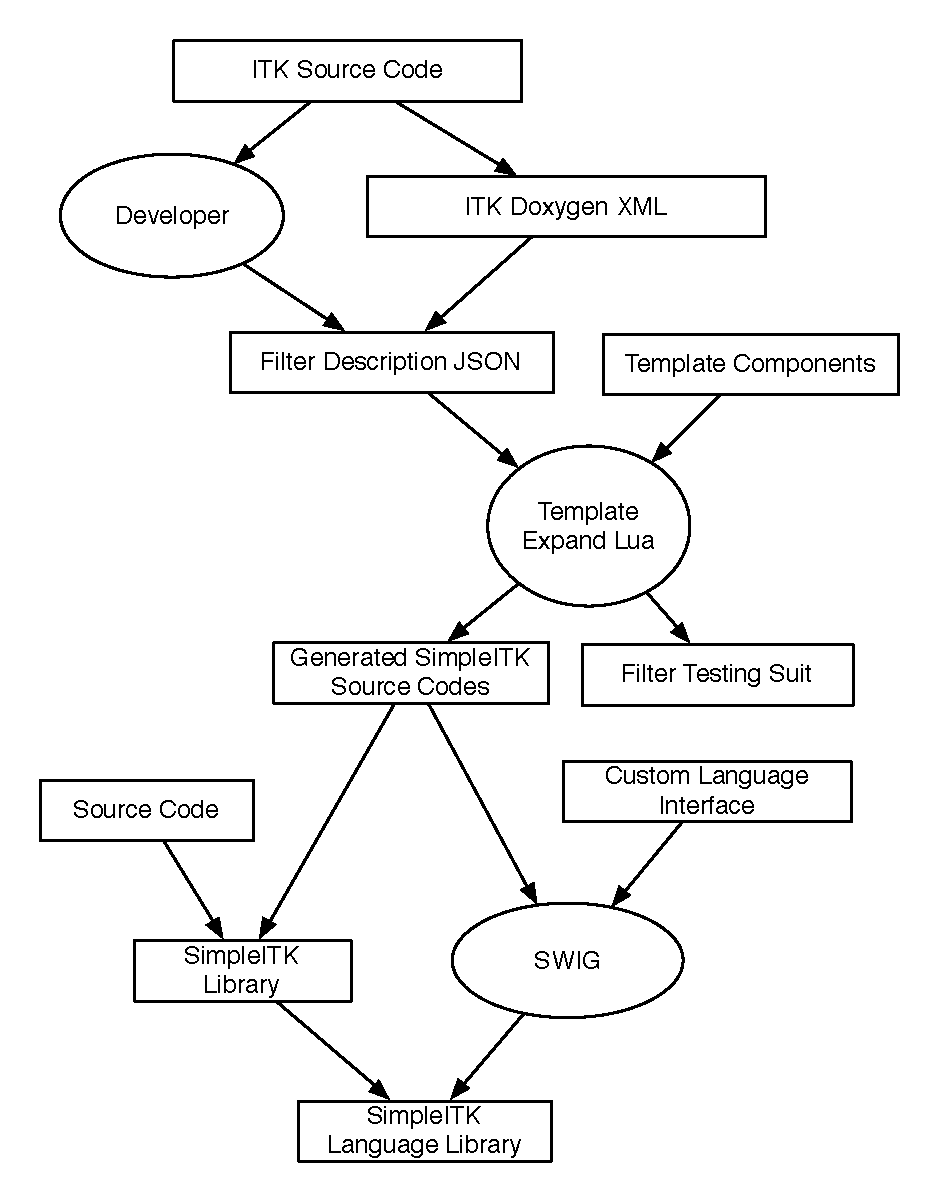
\includegraphics[width=8.5cm]{images/fig1_dataflow}
\end{center}
 \textbf{\refstepcounter{figure}\label{fig:01} Figure \arabic{figure}.}{ SimpleITK data flow diagram. }
\end{figure}

\begin{figure}
\begin{center}
\includegraphics[width=8.5cm]{images/fig2_t1t2image}
\end{center}
 \textbf{\refstepcounter{figure}\label{fig:02} Figure \arabic{figure}.}{ Axial cross sections of T1 (left) and T2 (right) MRI of a brain. }
\end{figure}

\begin{figure}
\begin{center}
\includegraphics[width=18cm]{images/fig3_seeds}
\end{center}
 \textbf{\refstepcounter{figure}\label{fig:03} Figure \arabic{figure}.}{ Segmentation seeds in T1. }
\end{figure}

\begin{figure}
\begin{center}
\includegraphics[width=18cm]{images/fig4_seg}
\end{center}
 \textbf{\refstepcounter{figure}\label{fig:04} Figure \arabic{figure}.}{ Ventricle segmentation. }
\end{figure}


\begin{figure}
\begin{center}
\includegraphics[width=8.5cm]{images/fig5_ventricle}
\end{center}
 \textbf{\refstepcounter{figure}\label{fig:05} Figure \arabic{figure}.}{ Volume rendering of ventricle. }
\end{figure}

\begin{figure}
\begin{center}
\includegraphics[width=8.5cm]{images/fig6_gold}
\end{center}
 \textbf{\refstepcounter{figure}\label{fig:06} Figure \arabic{figure}.}{ Slice from the gold bead volume. }
\end{figure}

\begin{figure}
\begin{center}
\includegraphics[width=8.5cm]{images/fig7_goldseg}
\end{center}
 \textbf{\refstepcounter{figure}\label{fig:07} Figure \arabic{figure}.}{ Gold bead segmentation results. }
\end{figure}

\begin{figure}
\begin{center}
\includegraphics[width=18cm]{images/fig8_goldvolume}
\end{center}
 \textbf{\refstepcounter{figure}\label{fig:08} Figure \arabic{figure}.}{ Volume rendering of labeled gold bead segmentation. }
\end{figure}

%\begin{figure}
%\begin{center}
%
\includegraphics[width=3.5cm]{logo2}% This is an *.eps file
%\end{center}
% \textbf{\refstepcounter{figure}\label{fig:02} Figure \arabic{figure}.}{ Enter the caption for your figure here.  Repeat as  necessary for each of your figures }
%\end{figure}


%%% Frontiers will add the figures at the end of the provisional pdf automatically %%%

%%% The use of LaTeX coding to draw Diagrams/Figures/Structures should be avoided. They should be external callouts including graphics.

\end{document}
